%%%%%%%%%%%%%%%%%%%%%%%%%%%%%%%%%%%%%%%%%%%%%%%%%%%%%%%%%%%%%%%%%%%%%%%%%%%%
\documentclass[a4j]{jarticle}

\usepackage{jsaisig}
% \usepackage{graphicx}
\usepackage[dvipdfmx]{graphicx}
\usepackage{subfigure}
\usepackage{multirow}
\usepackage{url}
% \usepackage{}

%%%%%%%%%%%%%%%%%%%%%%%%%%%%%%%%%%%%%%%%%%%%%%%%%%%%%%%%%%%%%%%%%%%%%%%%%%%

\begin{document}

% 和文タイトル
% \title{Find My Matesに向けた解法の提案と実機での性能評価}
% \title{RoboCup@Homeタスク:Find My Matesに向けた解法の提案とロボット実機での性能評価}
\title{RoboCup@Homeのヒューマンインタラクションタスク\\に向けた解法の提案}

% 英文タイトル
% \etitle{Solving RoboCup@Home Task: Find My Mates and Evaluation Using Domestic Standard Robot}
\etitle{Proposal for Solution of Human Interaction Task in RoboCup@Home}

% 著者名:
%	・各著者を\quad(全角空白)区切りで列挙
% 	・著者名の直後に\afil{所属番号}を追加→所属番号を上付で出力(\textsuperscript{所属番号}と同じ)
% 	 複数機関へ所属している場合は番号をカンマ区切りで列挙(下記著者2参照)
%  ・Corresponding Authorについては所属の後に\thanksを続け,連絡先を記入
%	・英文著者はカンマ区切りで列挙

\author{矢野 優雅\afil{1}%
	\thanks{連絡先:九州工業大学大学院生命体工学研究科人間知能システム工学専攻 \newline%
		      〒808-0135 福岡県北九州市若松区ひびきの2-4 \newline%
		      E-mail: yano.yuuga158@mail.kyutech.jp}\quad%
	松本 生弥\afil{1}
	福田 有輝也\afil{1}
	小野 智寛\afil{1,2}
	田向 権\afil{1,3}\\
	Yuga Yano\afil{1}, Ikuya Matsumoto\afil{1}, Yukiya Fukuda\afil{1}, Tomohiro Ono\afil{1,2}, and Hakaru Tamukoh\afil{1,3}}

% 所属
\affiliation{%
	\afil{1} 九州工業大学大学院生命体工学研究科\\
	\afil{1} Graduate School of Life Science and Systems Engineering, Kyushu Institute of Technology, Japan\\
	\afil{2} 日本学術振興会特別研究員DC\\
	\afil{2} Research Fellow of the Japan Society for the Promotion of Science\\
	\afil{3} ニューロモルフィックAIハードウェア研究センター\\
	\afil{3} Research Center for Neuromorphic AI Hardware, Kyushu Institute of Technology, Japan}

\abstract{
% Abstract (English) comes here.......................................................
ホームサービスロボットの技術発展を目的として,RoboCup@Homeという競技会が開催されている.
RoboCup@Homeでは,実際の家庭環境を模したフィールドを用いてタスクを行うことで,より現実に近い環境でロボットの性能を評価することができる.
% 本研究では,RoboCup@Homeのタスクの一つであるFind My Matesに向けて,満点を獲得するための手法を提案する.
% 本研究では,RoboCup@HomeのタスクであるFind My Matesに向けて,人物認識や音声認識を用いた手法を提案する.
本研究では,RoboCup@HomeのタスクであるFind My Matesを解くために,人物認識や音声認識を用いた動的環境でも動作する手法を提案する.
% また,提案した手法をロボットに実装し,2022年7月にバンコクで行われたRoboCup@Homeにて現地実験を行った.
% また,提案した手法をロボットに実装し,RoboCup@Homeにて現地実験を行った.
また,提案した手法をロボットに実装し,2022年7月にバンコクで行われたRoboCup@Homeにて性能評価を行った.
% 現地実験では満点を獲得し,提案手法の有効性を示した.
競技会では満点を獲得し,提案手法の有効性を示した.
競技中の様子は,\url{https://www.youtube.com/watch?v=ucoP8_j6Kig} にて公開している.
}

\maketitle
\thispagestyle{empty}

%%%%%%%%%%%%%%%%%%%%%%%%%%%%%%%%%%%%%%

\section{序論}
% テストと競技表記ゆれが起きそうなので,早いうちに確定させる
% \subsection{RoboCup@Home}
RoboCup@Home\cite{robocup_hp}は,ホームサービスロボットの技術発展を目的に開催されている国際的な競技会である.
本競技会では,人間とロボットの協調を目標の一つに掲げており,
音声認識や物体認識,ナビゲーションといったテストが動的環境下で行われている.
そのため,より現実に近い家庭環境でロボットの性能を評価することができ,多くの注目を集めている.
% The RoboCup@Home league aims to develop service and assistive robot technology with high relevance for future personal domestic applications. It is the largest international annual competition for autonomous service robots and is part of the RoboCup initiative. A set of benchmark tests is used to evaluate the robots’ abilities and performance in a realistic non-standardized home environment setting. Focus lies on the following domains but is not limited to: Human-Robot-Interaction and Cooperation, Navigation and Mapping in dynamic environments, Computer Vision and Object Recognition under natural light conditions, Object Manipulation, Adaptive Behaviors, Behavior Integration, Ambient Intelligence, Standardization and System Integration. It is colocated with the RoboCup symposium.
RoboCup@Homeには,Open Platform League,Domestic Standard Platform League(DSPL),Social Standard Platform Leagueという3つのリーグがある.
我々の参加しているDSPLでは,トヨタ自動車株式会社が開発したHuman Support Robot(HSR)\cite{hsr_paper}を標準機に採用しテストを行っている.
図\ref{overview_hsr}に,HSRの外観と搭載されている主なデバイスを示す.
\begin{figure}[ht]
  \centering
  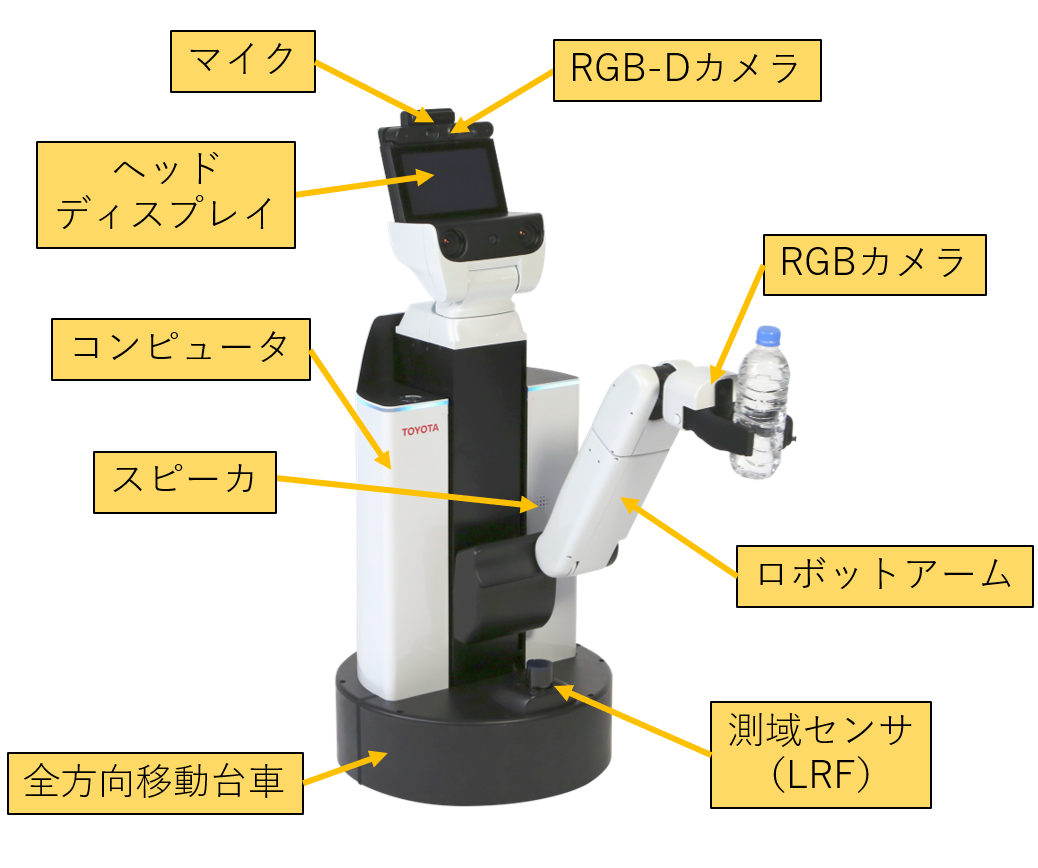
\includegraphics[width=6cm]{images/hsr/hsr_explain_ja.png}
  \caption{トヨタ自動車株式会社が開発したHSR}
  \label{overview_hsr}
\end{figure}
% HSRは移動台車やアームに加えて,RGB-Dカメラやマイクが搭載されており,認識を通して多様なヒューマンインタラクションを行うことができる.
HSRは移動台車やアームに加えて,RGB-Dカメラやマイクが搭載されているため,物体認識や音声認識を通して動的環境下においても多様な動作を実現できるロボットである.

本研究では,特にヒューマンインタラクションの性能をはかるFind My Mates(FMM)というタスクに向けて,その解法を提案する.
また,提案した手法をHSRに実装し,2022年7月にバンコクで行われたRoboCup@Homeにて性能評価を行った.
競技会では満点を獲得し,本手法の有効性を示した.
% しかし,課題も多く見つかったため,それらに対する考察も行う.
% RoboCup@Homeのタスクの一つであるFind My Mates(FMM)に着目する.
% FMMは人物認識や音声認識が必要となるタスクであり,特にヒューマンインタラクションの性能をはかることができる.

% 2ページ目の先頭に持ってくるため
\begin{figure*}[ht]
  \centering
  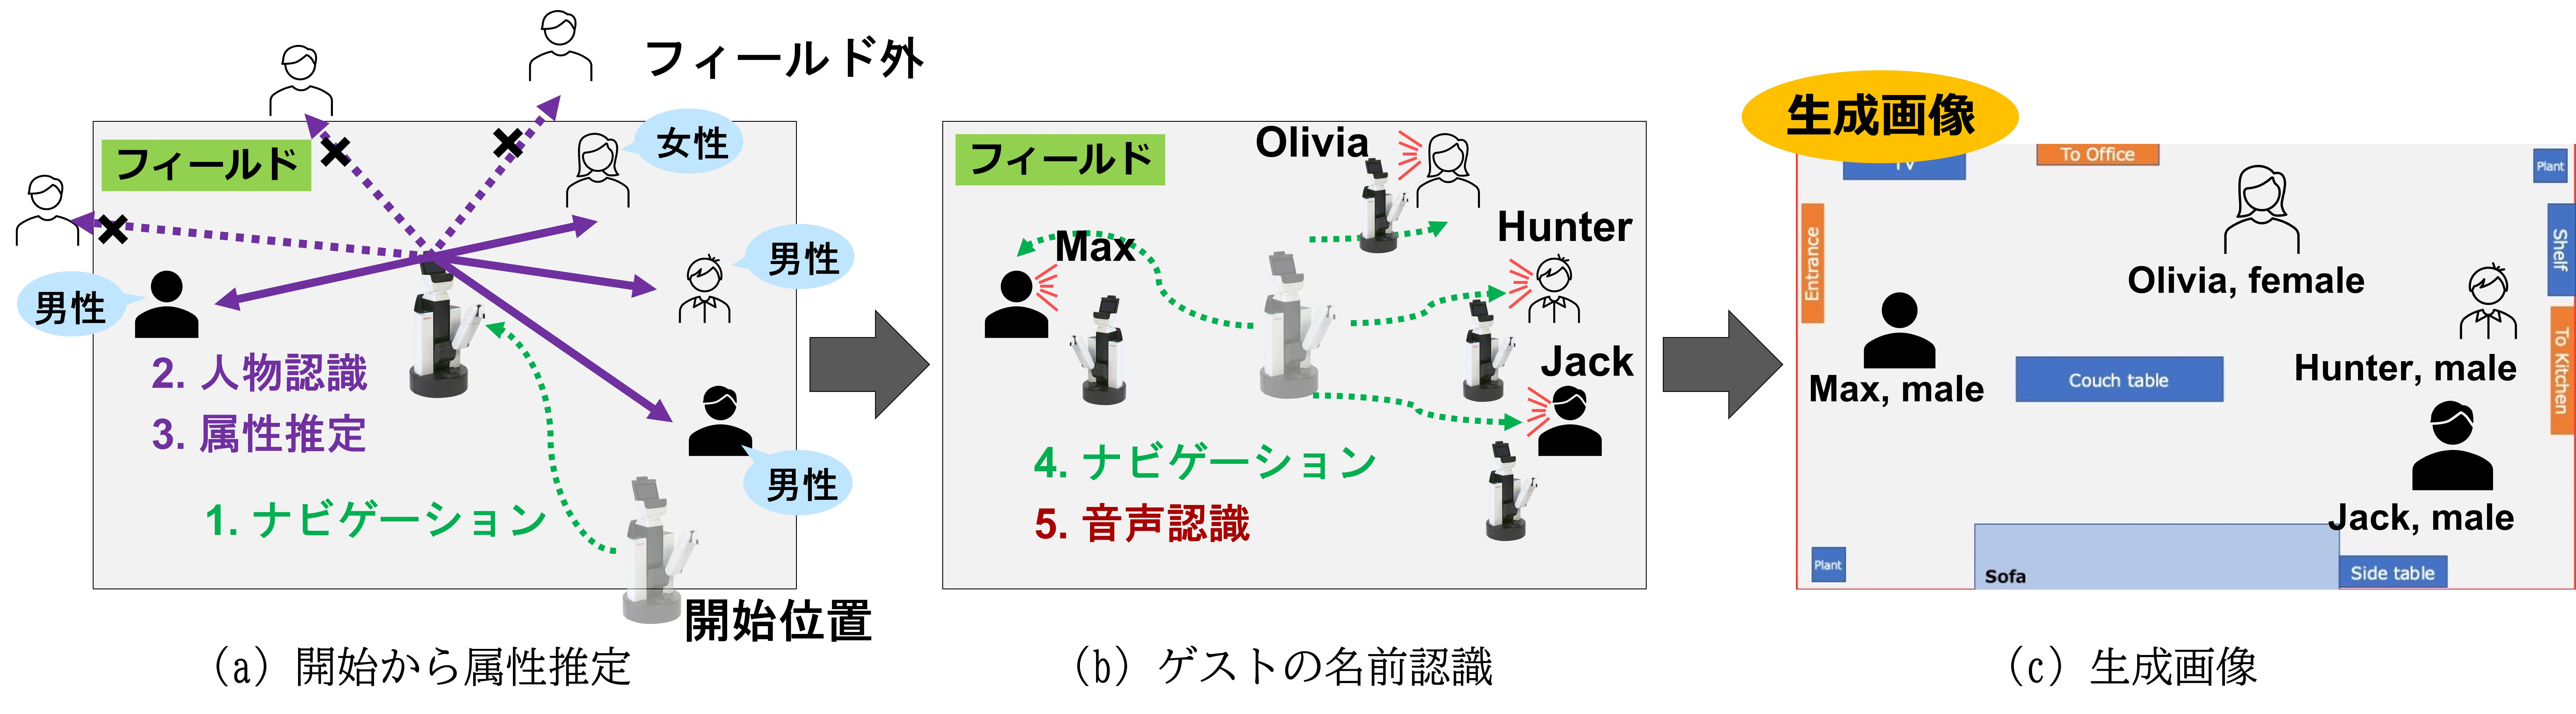
\includegraphics[width=16cm]{images/FMM/solution_overview_yoko_yy2_cap_comp.jpg}
  \caption{提案したFMMの解法}
  \label{solution_overview}
\end{figure*}

% \subsection{Find My Mates}
% 本章では,RoboCup@Homeで行われるFind My Mates(FMM)というタスクについて述べる.
% FMMでは,4人のゲストが1人のホストを訪れたという状況を想定している.
% % しかし,ホストはゲストの名前のみを知っているがその他の情報は何も知らない.
% FMMは,1人のホストの家に訪れた4人のゲストをロボットが探し,その場所,名前に加えて人物の特徴をホストに報告するというタスクである.
% そのため,人物を3次元的に認識する技術と,それぞれのゲストの特徴を抽出する属性推定の技術が必要になる.
% 更に,ロボットは事前にゲストの名前を知らされていないため,音声認識を通してゲストの名前を知る必要がある.

% \section{RoboCup@Home}

\section{Find My Mates}
本節では,RoboCup@Homeで行われるタスクの一つであるFMMについて述べる.
% FMMの得点表を表\label{points_table_fmm}に示す.
FMMでは4人のゲストと1人のホストが登場し,ホストの家にゲスト全員が訪れたという状況を想定している.
% しかし本タスクでは,ホストはゲストの名前のみを事前に知らされているが,それぞれの外見や特徴については何も知らされていない.
しかし本タスクでは,ホストはゲストの外見や特徴については何も知らされておらず,名前のみを知らされている.
そのため,ロボットが家に訪れたゲストを見つけ出し,顔や特徴,また部屋のどこにいるのかをホストに伝えることがFMMのメインゴールである.
FMMの得点表を表\ref{points_table_fmm}に示す.

FMMを遂行するためには,3次元位置を含む人物認識に加えて,人物の特徴を推定する技術が必要になる.
また,ゲストの名前を取得するためには,音声認識の技術も不可欠である.
このように,FMMはヒューマンインタラクションのために必要な技術を包括的に評価することができるタスクである.
% ただし,人物認識や音声認識ができなかった場合においては,ゲストからロボットに近づくことや,QRコード等による音声認識のバイパスも認められている.

% そのため,FMMを達成することで実環境においても

\begin{table}[h]
	\centering
	\caption{FMMの得点表}
	\label{points_table_fmm}
	\begin{tabular}{cccc}
		\hline
		動作項目                                                       & 回数 & 点/回数         & 合計点  \\ \hline
		\multicolumn{4}{c}{\textbf{メインゴール}}                                                   \\ \hline
		ゲストの位置報告                                                   & 2  & 100          & 200  \\ \hline
		\begin{tabular}[c]{@{}c@{}}明示的に\\ 位置を報告する\end{tabular} & 2  & 50           & 100  \\ \hline
		\begin{tabular}[c]{@{}c@{}}ゲストの\\ 特徴報告\end{tabular}        & 2  & 150          & 300  \\ \hline
		\multicolumn{4}{c}{\textbf{ボーナス}}                                                   \\ \hline
		\begin{tabular}[c]{@{}c@{}}3人目の\\ ゲストも報告\end{tabular}      & 1  & 150 & 150  \\ \hline
		\begin{tabular}[c]{@{}c@{}}3人目のゲストの\\ 特徴も報告\end{tabular}   & 1  & 250          & 250  \\ \hline
		\multicolumn{4}{c}{\textbf{減点対象}}                                                     \\ \hline
		\begin{tabular}[c]{@{}c@{}}ゲストから\\ 合図をもらう\end{tabular}     & 2  & -75          &      \\ \hline
		\begin{tabular}[c]{@{}c@{}}ゲストの位置を\\ 教えてもらう\end{tabular}   & 2  & -75          &      \\ \hline
		\begin{tabular}[c]{@{}c@{}}ゲストから\\ ロボットに近づく\end{tabular}   & 2  & -150         &      \\ \hline
		\multicolumn{3}{c}{合計}                                                         & 1000 \\ \hline
	\end{tabular}
\end{table}

\subsection{登場人物について}
\label{about_name_list}
RoboCup@Homeでは,タスクに登場する人物はボランティアから選出され,トライごとに変化する.
また,登場人物は自分の本名を使用するのではなく,事前に公開されている名前リストよりランダムに決定される.
この名前リストには,アメリカで一般的に使用されている名前から選出した男女11個ずつの名前が含まれている.
しかし,名前のみで男女の判別ができないように,男女で共通している名前が複数存在する.
そのため,性別については別の手段を用いて認識する必要がある.


\section{提案手法}
本章では,FMMで満点を獲得するための解法と,HSRに実装した機能について述べる.
% FMMでは部屋に移動した後,4人のゲストを見つける必要がある.
\begin{figure}[t]
  \centering
  \subfigure[RGB画像での認識結果]{
  	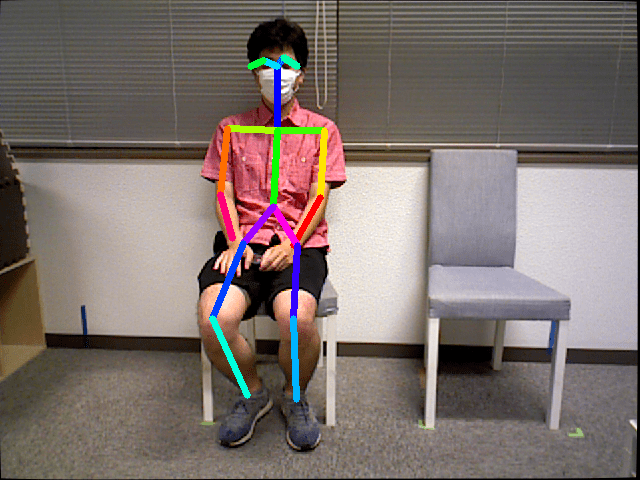
\includegraphics[height=3cm]{images/human_recognition/image_comp.png}
	\label{human_estimation_image}
	% \caption{RGB画像での認識結果}
  }
  % \subfigure[Depth画像と合わせた3次元の位置推定]{
  \subfigure[3次元の位置推定]{
  	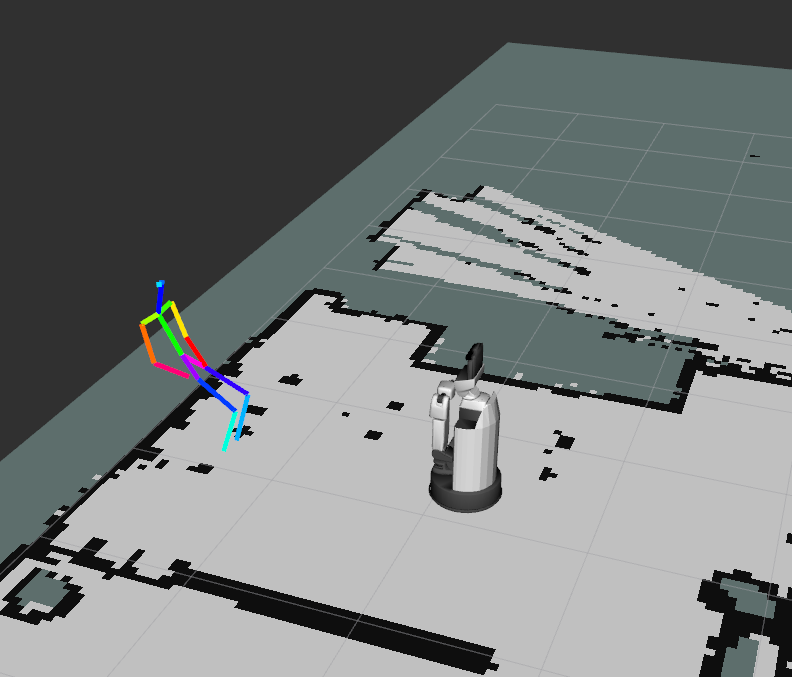
\includegraphics[height=3cm]{images/human_recognition/ss_4_trim.png}
	\label{human_estimation_pc}
	% \caption{Depth画像と合わせた3次元の位置推定}
  }
  \caption{人物位置推定アルゴリズム}
  \label{human_estimation_explain}
\end{figure}

\subsection{FMMに向けた解法}
% 私達はFMMで満点を獲得するために,次のような手法を提案する.
% 提案手法の概要を図\ref{solution_overview}に示す.
我々はFMMで満点を獲得するために,図\ref{solution_overview}に示す手法を提案する.
始めに,ロボットを部屋の中央までナビゲーションさせ,部屋全体を見渡しながら人物認識を用いて4人のゲストを見つける.
% 人物の認識にはRGB画像を用いるが,Depth画像も用いることで,認識した人が部屋のどこにいるのかも同時に算出する.
% 認識にはRGB画像のみを用いるが,この時RGB-DカメラのDepth情報を活用することで,それぞれのゲストの位置も同時に算出する.
認識にはRGB画像のみを用いるが,Depth情報も活用することでそれぞれのゲストの位置も同時に算出する.
% 次に,認識した人がエリア内のどこにいるかの判定を行う.これには,大きく2つの理由がある.
% 1つは,ロケーション報告に用いるためであり,
% もう1つは,フィールド周囲の観客の誤認識を防ぐためである.
次に,算出したゲストの位置を基に,各ゲストの正面までナビゲーションを行い,音声認識を用いて名前を聞く.
% ここで,音声認識結果が得られなかった場合,QRコードを用いてゲストの名前を取得する.
% 更に属性推定を用いて,ゲストの性別を推定する.
更にClass-Specific Residual Attention \cite{CSRA}という属性推定手法を用いて,ゲストの性別を推定する.

最後に,獲得したすべての情報(ゲストの画像,位置,名前,性別)を集約した1枚の画像を生成し,HSRの
ヘッドディスプレイに表示することでホストに伝える.
本手法で生成する画像を図\ref{solution_overview} (c)に示す.
このように,フィールドと各ゲストの情報をまとめて表示するため,メインゴールとボーナスを同時に達成できる.
% この生成画像ではフィールドを簡易的な画像で表現し,その上にゲストを示しているため,明示的に位置を報告することができている.
% また,4人同時に報告が行えるため,メインゴールとボーナスを同時に獲得できる.


\subsection{音声認識}
近年ではスマートフォンやスマートスピーカーなどの普及により,クラウドを用いた音声認識の研究が盛んである\cite{google_speech_api, amazon_speech_api}.
しかし,RoboCup@Homeでは会場のネットワークが不安定である場合が想定され,クラウド上での安定した音声認識は困難である.
また,ネットワークの課題は一般の家庭環境においても想定されるものであるため,オフラインでの音声認識技術が必要である.
% を利用することは非常に有効である.
そこで本研究では,vosk\cite{vosk_hp}と呼ばれるオフライン音声認識手法を用いる.

% 更に,voskは認識する単語リスト(辞書)を設定することで,辞書にない単語の認識をはじくことができる.
更に,voskは認識する単語リスト(辞書)を指定することで,辞書にない単語を認識から除くことができる.
\ref{about_name_list}節で述べた通り,RoboCup@Homeではタスクに登場する人物の名前リストが公開されている.
そのため,名前リストを基に辞書を作成しvoskに適用することで,認識精度向上を図る.

また,RoboCup@Homeでは音声認識をQRコードによってバイパスすることが認められている.
そこで,音声認識に失敗した場合は自動的にQRコードによる認識に切り替え,名前を取得する.
% 本研究では,音声認識を次のように実装している.
% まず,HSRのヘッド部に搭載されているマイクを用いて,音声認識を開始したタイミングから一定時間録音を行う.
% 次に,録音した音声をPC側へRobot Operating System(ROS)\cite{ros_wiki}を介して送信する.
% しかし,ROSには音声ファイルをそのまま扱うメッセージ型がないため,本研究では音声ファイルをnumpy形式に変換して送信する.
% % ここで,ROSには音声ファイルをそのまま送信できるメッセージ型がないため,音声ファイルをnumpyの配列に読み直して送信を行う.
% PC側では,受信したnumpyの配列から音声ファイルを再構築し,音声認識を行う.
% 音声ファイルをROSで通信したことも書く.
% 音声認識を一定時間で行っていることも書く
% 音声認識の結果の評価があっても面白い
% 一回でも認識できなかったら,そのタスク中は音声認識をあきらめる事もかいておくべき

% \subsubsection{辞書設定}
% % RoboCup@Homeでは,タスクに登場する人物は本名を使用するのではなく,
% % 事前に公開している名前リストから毎回ランダムに決定され名前を割り当てられる.
% % この名前リストには,男性用と女性の用の名前が約10個ずつ用意されている.
% % ただし,名前だけで性別の区別ができないようにするために,男性と女性で共通している名前も存在する.
% \ref{about_name_list}節で述べた通り,RoboCup@Homeではタスクに登場する人物の名前リストが公開されている.
% そのため,名前リストに含まれる単語のみを認識すればよい.
% そこで,名前リストを基に辞書を作成し,辞書に含まれる単語のみを認識
% そこで本研究では,名前リストを基にした辞書を作成し,voskに適用させることで音声認識の精度向上を図る.
% % ここ定量的な表現に直す
% % 辞書を設定していない場合では,名前を話してもまったく違う単語として認識されることがほとんどであったが,
% % 辞書設定をすることで認識率は飛躍的に向上した.
% 辞書を設定していない場合では,発話した名前が別の単語として認識されることが多かったが,辞書設定をすることで誤認識が減少した.

\subsubsection{ノイズ除去}
RoboCup@Homeは実際の家庭環境を模したフィールドで行われるが,実際の家庭環境と異なる点もある.
その一つが,周囲の外音(ノイズ)である.
RoboCup@Homeには多くの観客がおり,また他のリーグも同時に行われているため,実際の家庭環境では見られないようなノイズが発生する.
さらに,RoboCup@Home会場でのノイズの特性は大会ごとに異なり,現地での調整が必要である.
そのため,ノイズ除去の強度をパラメータで容易に調整可能なノイズ除去\cite{sainburg2020finding}を音声認識の前段に組み込んでいる.
% 本ノイズ除去の手法は,ノイズ除去の強度をパラメータで容易に変化させることができる.
% 本ノイズ除去の手法は実装が容易であり,ノイズ除去の強度も変化させることができるため採用した.
% 本研究では,音声認識の精度を高めるために,ノイズ除去\cite{sainburg2020finding}を音声認識の前段に組み込んでいる.
% これに定量的な実験結果を載せてもいいと思う

% \subsection{音声認識の性能評価}
% RoboCup@Homeで使用される名前は,アメリカで一般的に用いられる名前からランダムに決定される.
% そこで,アメリカで一般的に使用されている名前から男女それぞれ名前を11個選出し,本研究で作成した音声認識の精度を検証した.
% % 検証はノイズの大きな環境で行い,話者とノイズの環境を変化させながらそれぞれ4度ずつ読み上げて検証を行った.
% 検証データとして,RoboCup@Home会場で起こるノイズを再現した環境で録音し,各名前4回ずつの計88データを作成した.
% % 検証のための音声データは,RoboCup会場で起こりやすいノイズ環境を再現して,話者やノイズの強弱を変化させながら4度づつ読み上げて録音を行った.
% % 検証データは
%
% 表\ref{voice_recognition_result}に,ノイズ除去を行った場合と辞書指定を行った場合における認識結果を示す.
% 辞書指定を行い,ノイズ除去を行った手法が最も精度が高くなっていることが確認できた.
% \begin{table}[ht]
% 	\centering
% 	\caption{音声認識の精度}
% 	\begin{tabular}{|c|c|c|}
% 	\hline
% 	辞書指定                & ノイズ除去 & 認識精度(\%)          \\ \hline
% 	\multirow{2}{*}{なし} & なし    & 13.6          \\ \cline{2-3}
% 	                    & あり    & 10.2          \\ \hline
% 	\multirow{2}{*}{あり} & なし    & 69.3          \\ \cline{2-3}
% 	                    & あり    & \textbf{71.6} \\ \hline
% 	\end{tabular}
% 	\label{voice_recognition_result}
% \end{table}

\subsection{人物認識}
% \begin{figure}[t]
%   \centering
%   \subfigure[RGB画像での認識結果]{
%   	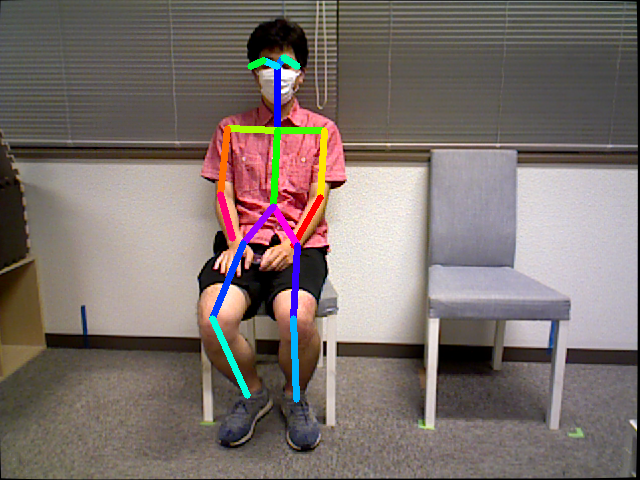
\includegraphics[height=3cm]{images/human_recognition/image.png}
% 	\label{human_estimation_image}
% 	% \caption{RGB画像での認識結果}
%   }
%   % \subfigure[Depth画像と合わせた3次元の位置推定]{
%   \subfigure[3次元の位置推定]{
%   	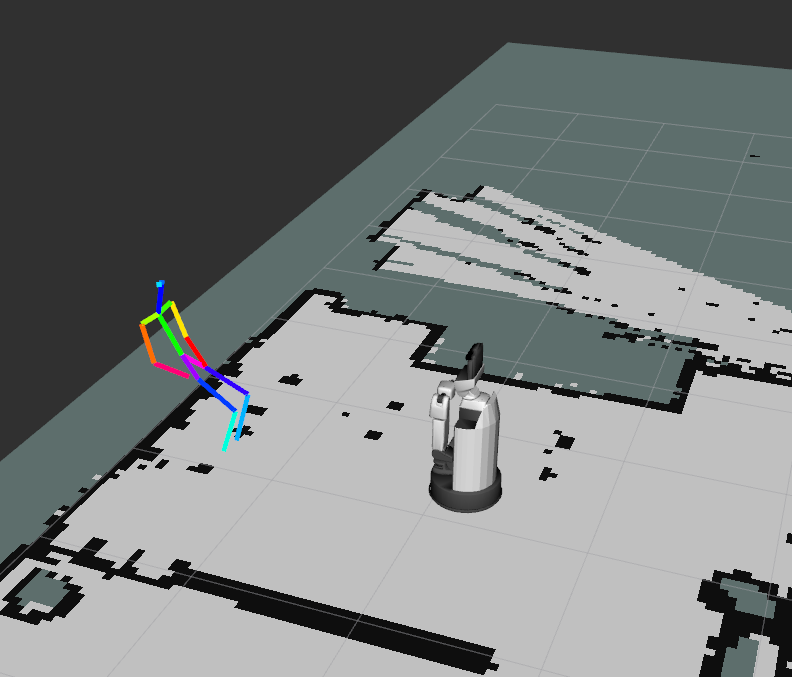
\includegraphics[height=3cm]{images/human_recognition/ss_4_trim.png}
% 	\label{human_estimation_pc}
% 	% \caption{Depth画像と合わせた3次元の位置推定}
%   }
%   \caption{人物位置推定アルゴリズム}
%   \label{human_estimation_explain}
% \end{figure}
本研究では人物認識の手法にLightweight Human Pose Estimation\cite{light-openpose}を用いた.
本手法は処理が非常に軽量であり,CPUでも高速に動作する手法である.
% 今回使用したPCでは,x fpsで動作しており,HSRのカメラ周期と同等な速度である為,リアルタイム動作を実現できていると言える.
% 本手法を用いることで,図3 (a)に示すように,HSRより取得したRGB画像から人物認識を行うことができる.
本手法を用いることで,図3 (a)に示すように,RGB画像から人物認識を行うことができる.
次に,RGB画像における認識結果と,Depth画像を合わせることで,人物の3次元位置推定を行う.
図3 (b)に,人物の3次元位置推定を行った結果を示す.
% 本研究では,人物を3次元的に認識する必要があるため,RGB画像から人物認識を行った後,
% 認識位置のDepth画像を参照することで,3次元的な位置を推定する.
% 図\ref{human_estimation_explain}に,人物の3次元的な位置推定を行った結果を示す.
% \begin{figure}[t]
%   \centering
%   \subfigure[RGB画像での認識結果]{
%   	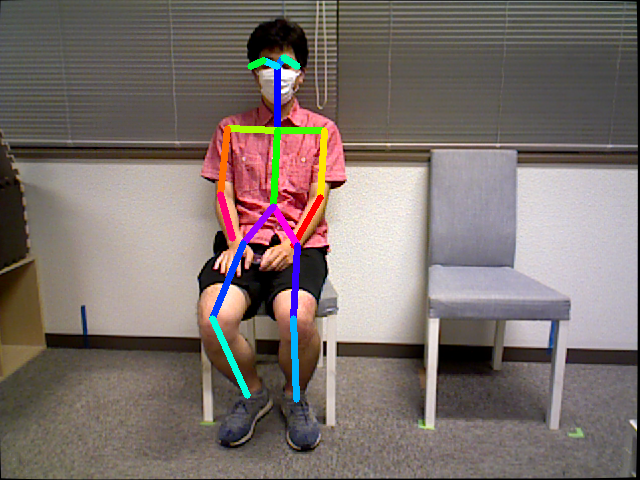
\includegraphics[height=3cm]{images/human_recognition/image.png}
% 	\label{human_estimation_image}
% 	% \caption{RGB画像での認識結果}
%   }
%   % \subfigure[Depth画像と合わせた3次元の位置推定]{
%   \subfigure[3次元の位置推定]{
%   	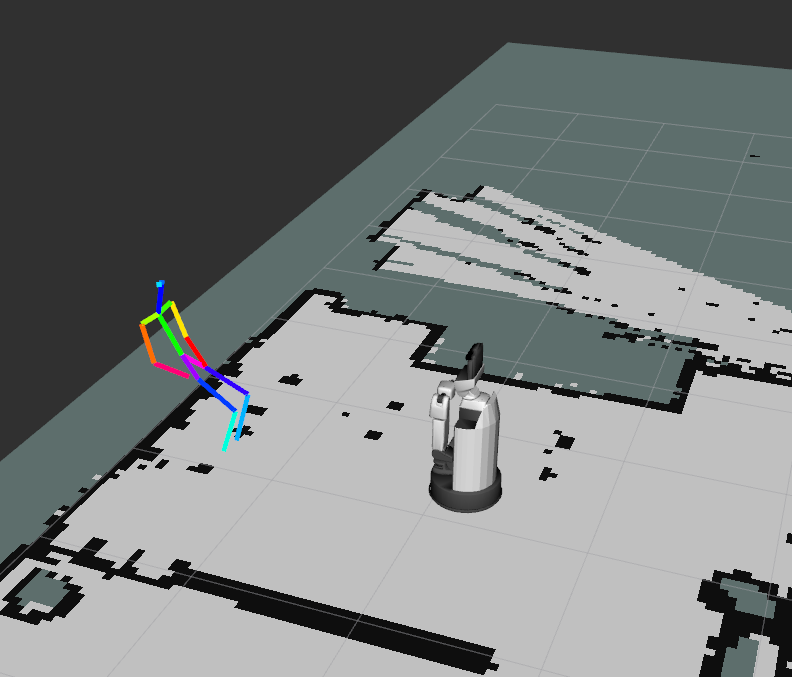
\includegraphics[height=3cm]{images/human_recognition/ss_4_trim.png}
% 	\label{human_estimation_pc}
% 	% \caption{Depth画像と合わせた3次元の位置推定}
%   }
%   \caption{人物位置推定アルゴリズム}
%   \label{human_estimation_explain}
% \end{figure}

\subsection{ゲストの位置報告}
% FMMでは,認識した人物をホストに伝える必要があるが,この際に考慮すべきこととして,
% 認識した人が本当に部屋の中にいる人なのか,部屋の中のどこにいるのかを識別する必要がある.
FMMでは,認識した人物の位置をホストに伝えるために,認識した人物が部屋の中のどこにいるのかを識別する必要がある.
% そこで本研究では,事前にrtabmap\cite{rtabmap}を用いて作成したマップに対してjsonファイルを用いて意味づけを行う.
% そこで本研究では,事前にrtabmap\cite{rtabmap}を用いて作成したマップに対して意味づけを行う.
そこで本研究では,Simultaneous Localization and Mappingを用いて事前に作成したマップに対して意味づけを行う.
RoboCup@Homeではフィールドの配置が事前に公開されるため,部屋の内外と椅子などの家具がどの位置にあるのかという情報も含めて意味づけを行う.
図3に示した3次元の人物認識に対して,フィールドの意味づけを行った結果を図\ref{human_where_map}に示す.
% と,フィールド内のどこに椅子があるのかといった家具の情報も付加する.
% またRoboCup@Homeでは,事前に部屋の形が公開されるため部屋の中のどこに椅子があるのかという意味づけも行う.
% 人物のフィールド内判定と,位置推定の結果を図\ref{human_where_map}に示す.
\begin{figure}[t]
  \centering
  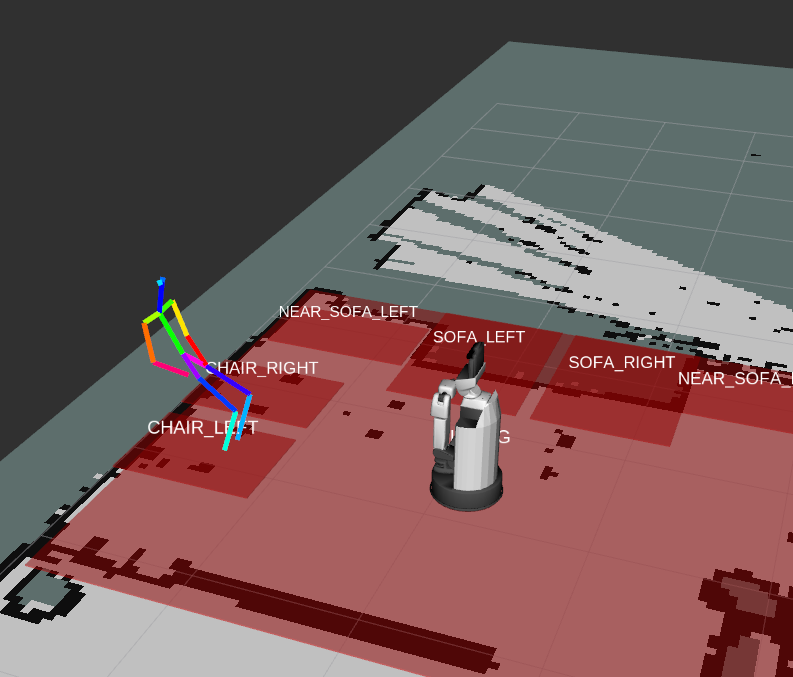
\includegraphics[width=5cm]{images/human_recognition/ss_5_trim.png}
  \caption{図3で認識した結果に意味づけを行った結果}
  \label{human_where_map}
\end{figure}
この場合では,ゲストはフィールド内の左側の椅子に座っていると正しく判定している.

%%%%%%%%%%%%%%%%%%%%%%%%%%%%%%%%%%%%%%

% \section{現地実験概要}
\section{競技概要}
\begin{figure}[ht]
  \centering
  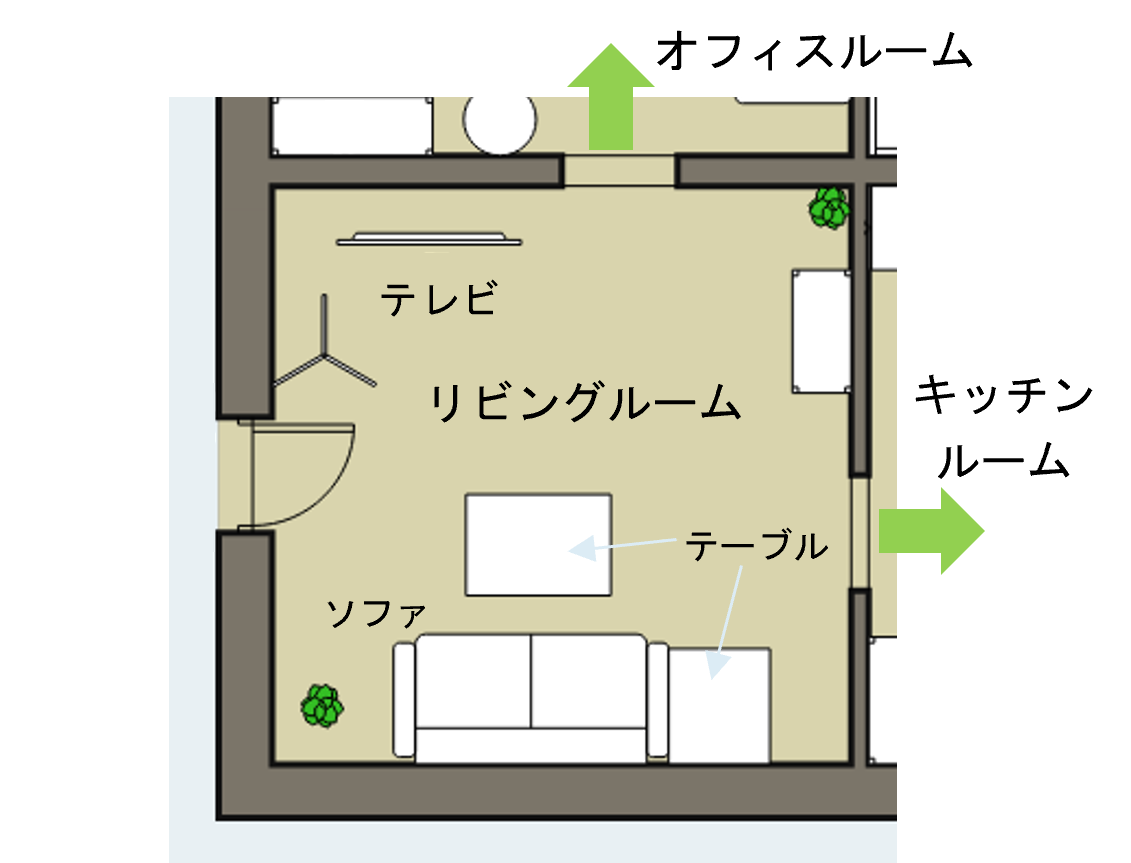
\includegraphics[width=5cm]{images/robocup/arenaBangkok_rotate_trim_yy2.png}
  % \caption{バンコクで開催されたRoboCup@Home2022で使用されたフィールド}
  \caption{RoboCup@Home2022で使用されたフィールド}
  \label{robocup_field}
\end{figure}
\begin{figure}[ht]
  \centering
  \subfigure[1度目のトライ]{
  	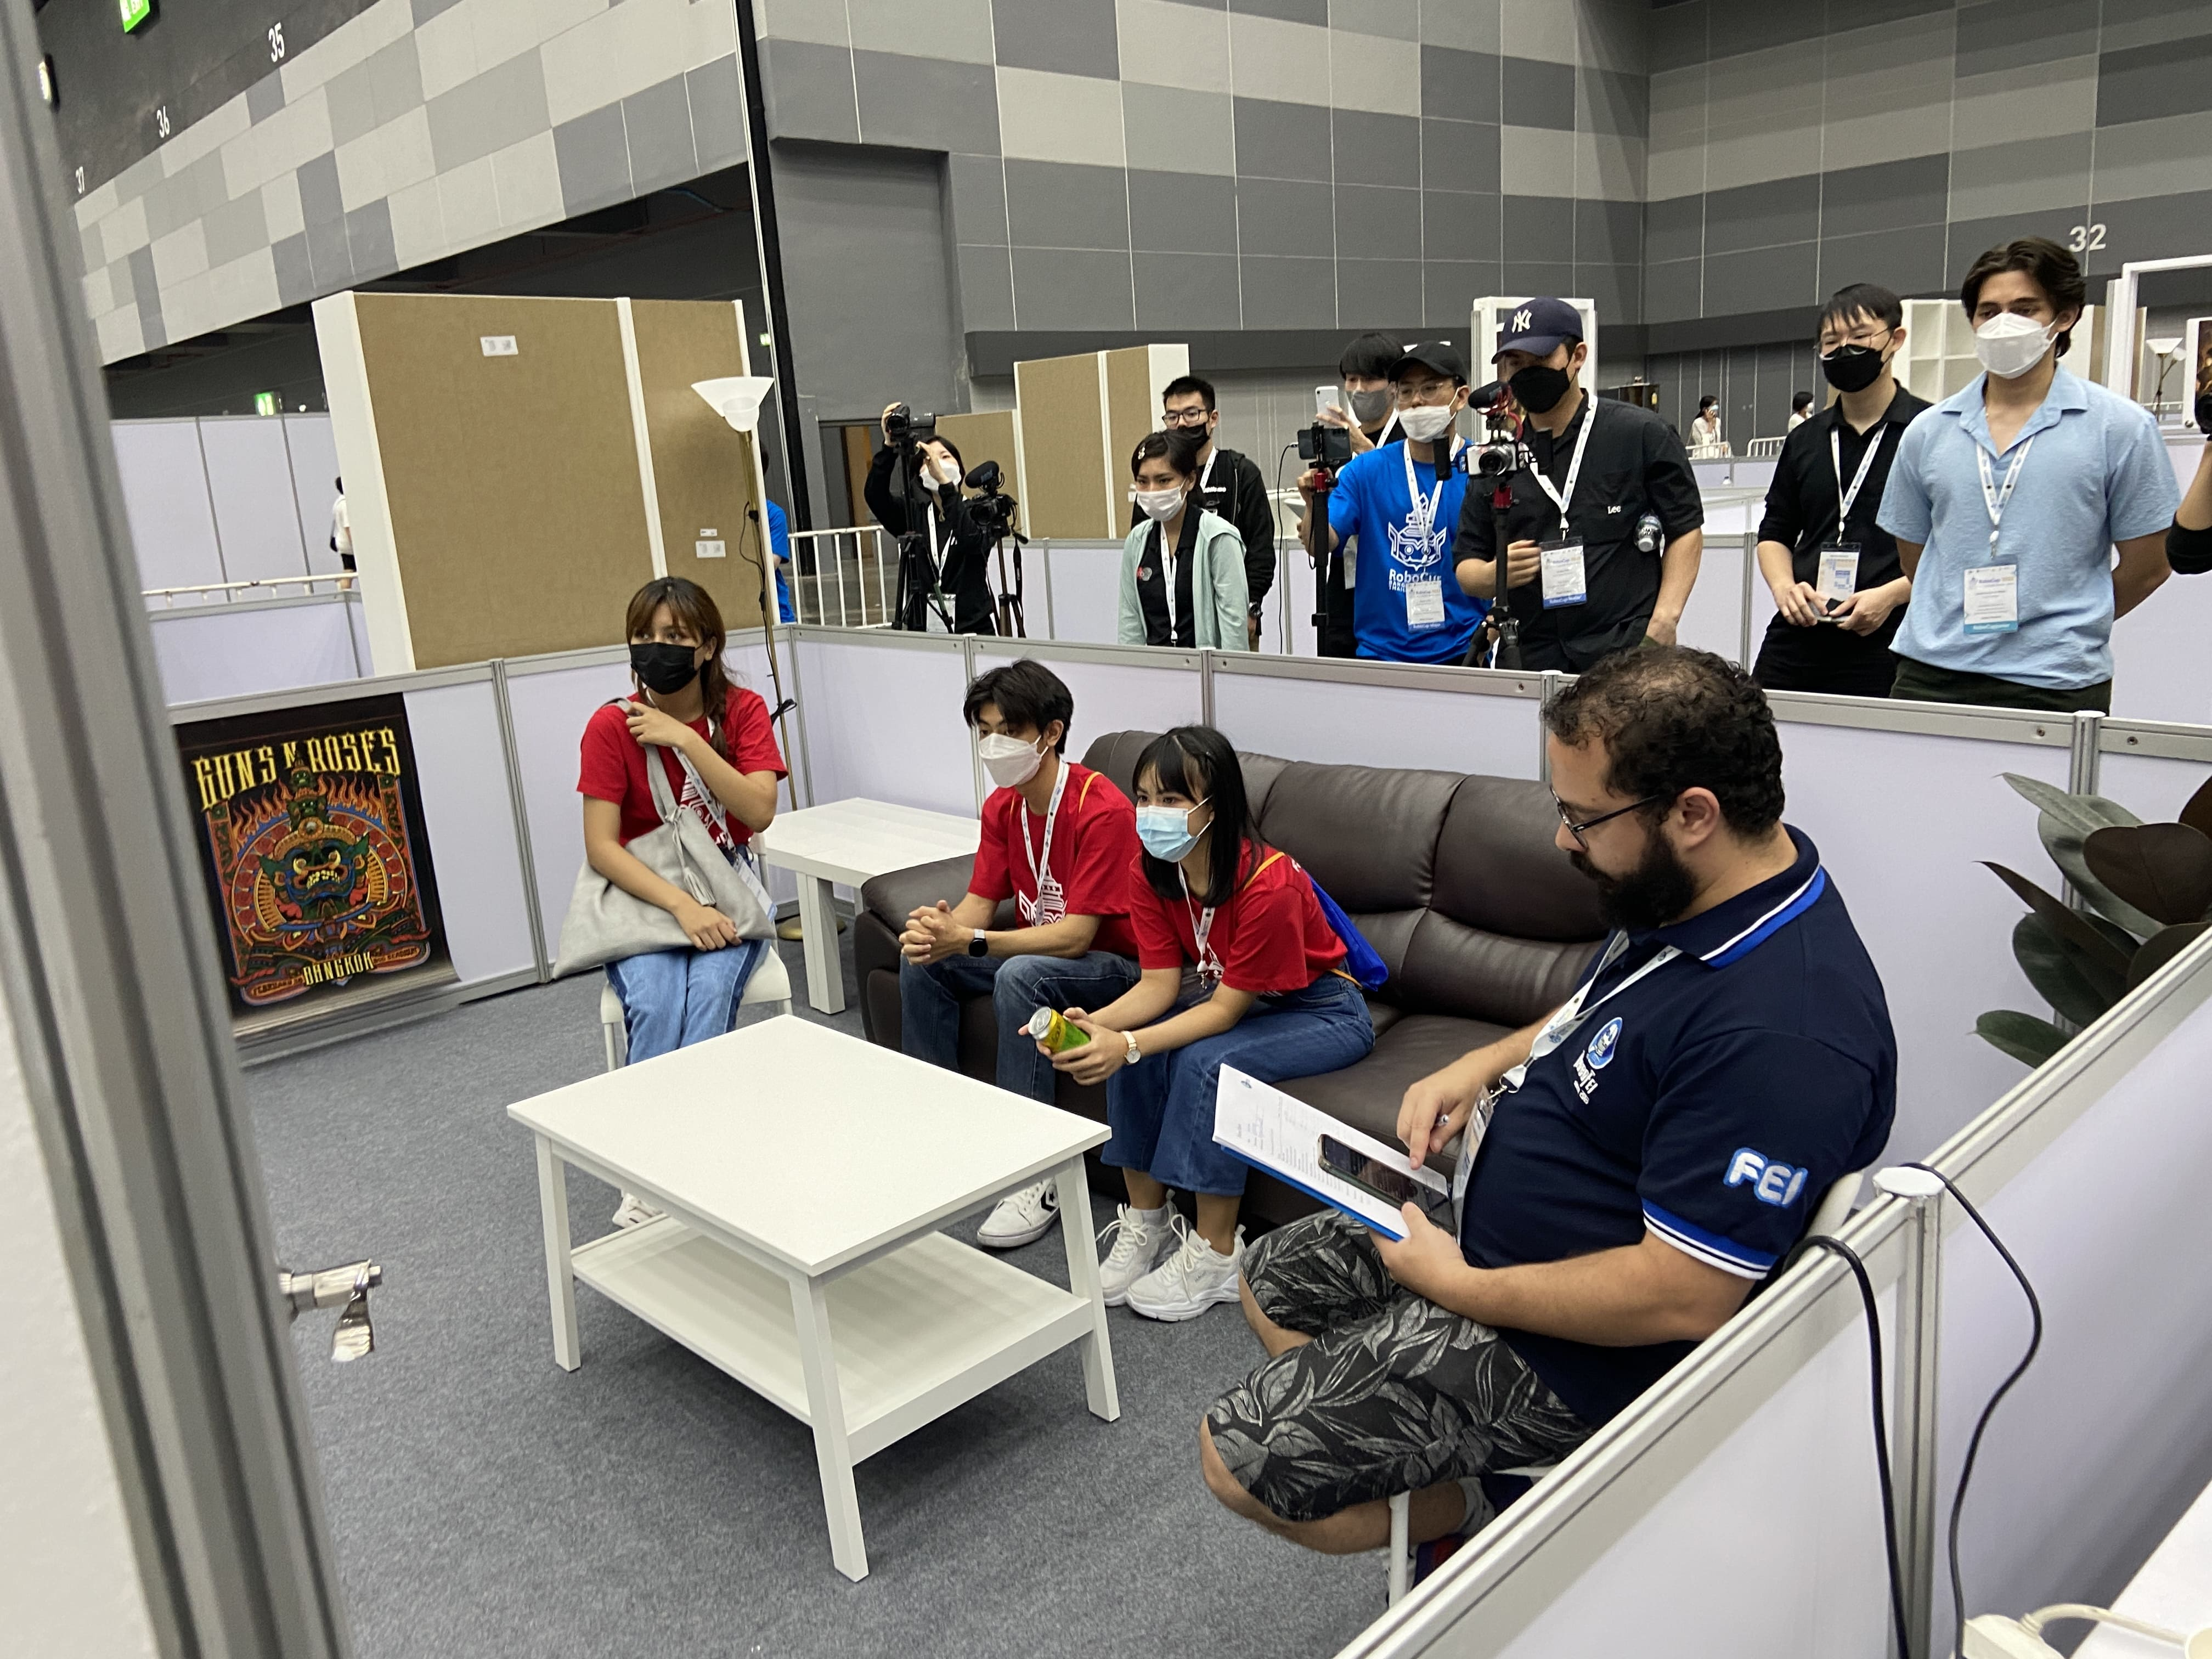
\includegraphics[height=2.2cm]{images/robocup/FMM_onsite_overview_1_comp.jpg}
  	\label{1st_trial_FMM}
  }
  \subfigure[2度目のトライ]{
  	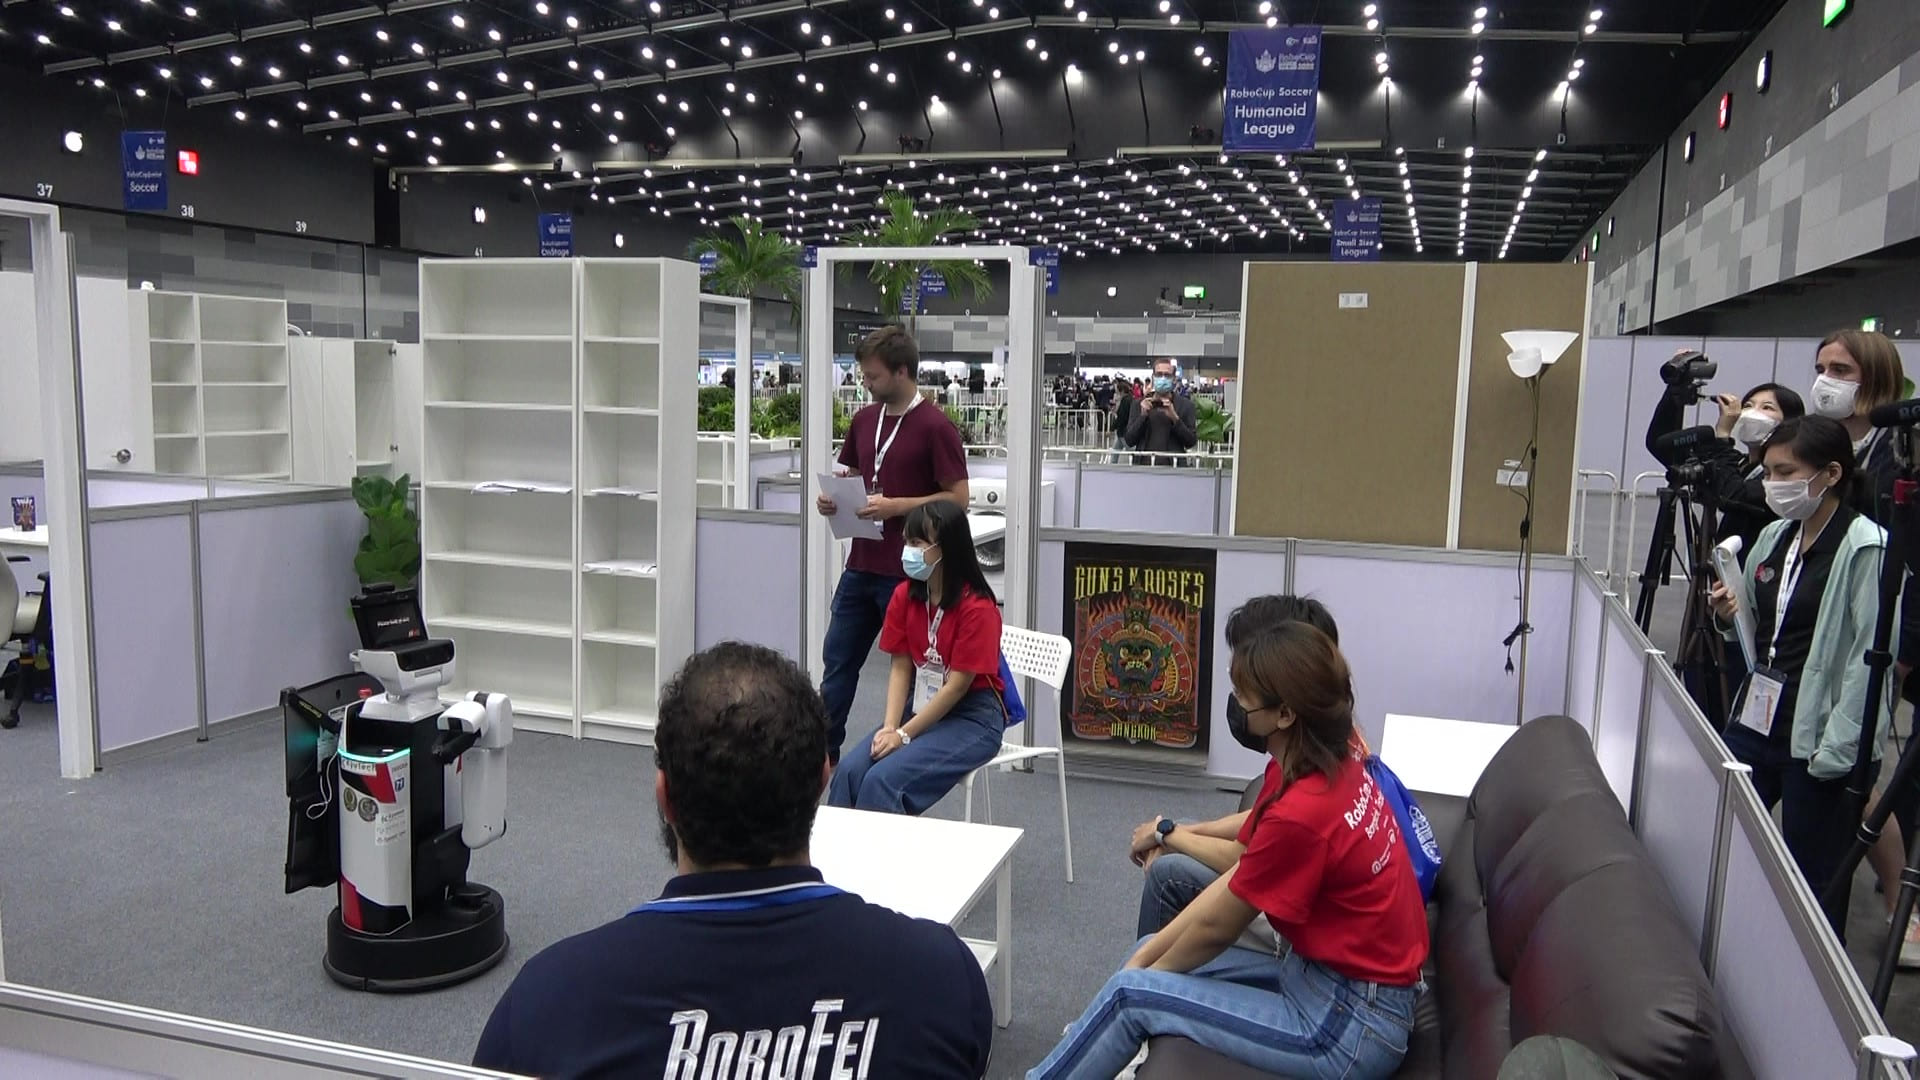
\includegraphics[height=2.2cm]{images/robocup/FMM_onsite_overview_3_comp.jpg}
  	\label{2nd_trial_FMM}
  }
  % 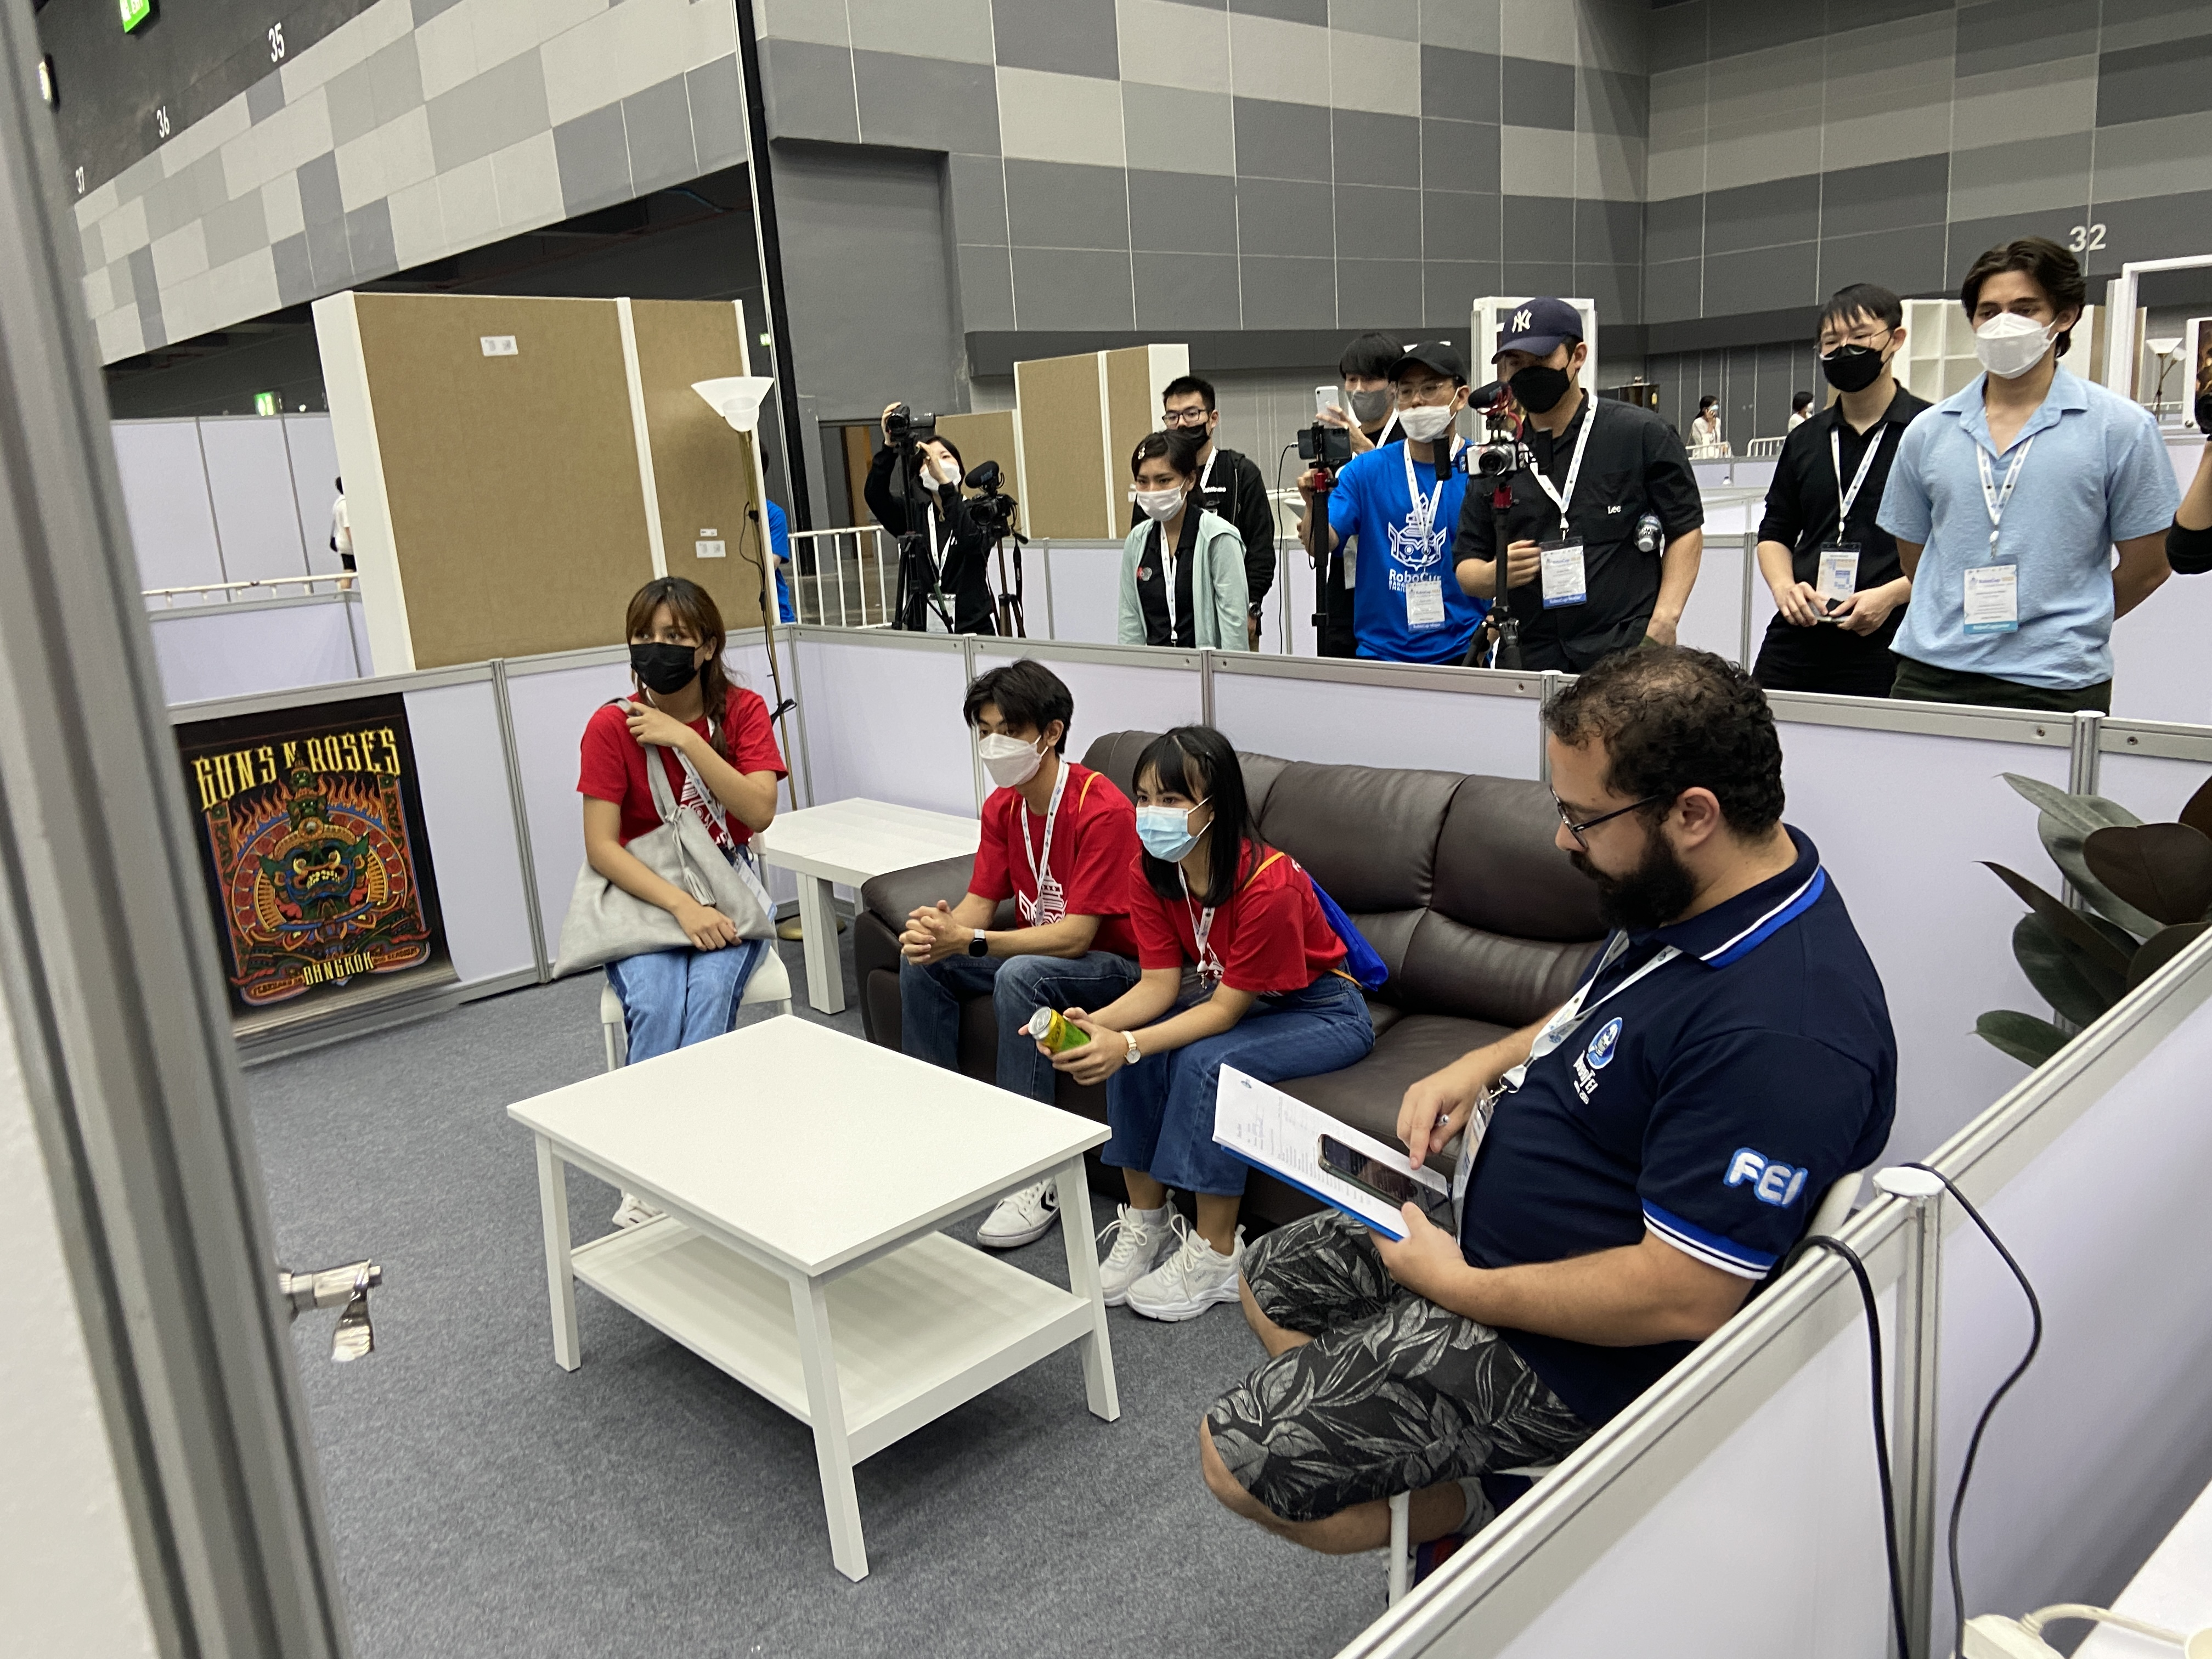
\includegraphics[height=2.2cm]{images/robocup/FMM_onsite_overview_1.jpg}
  % 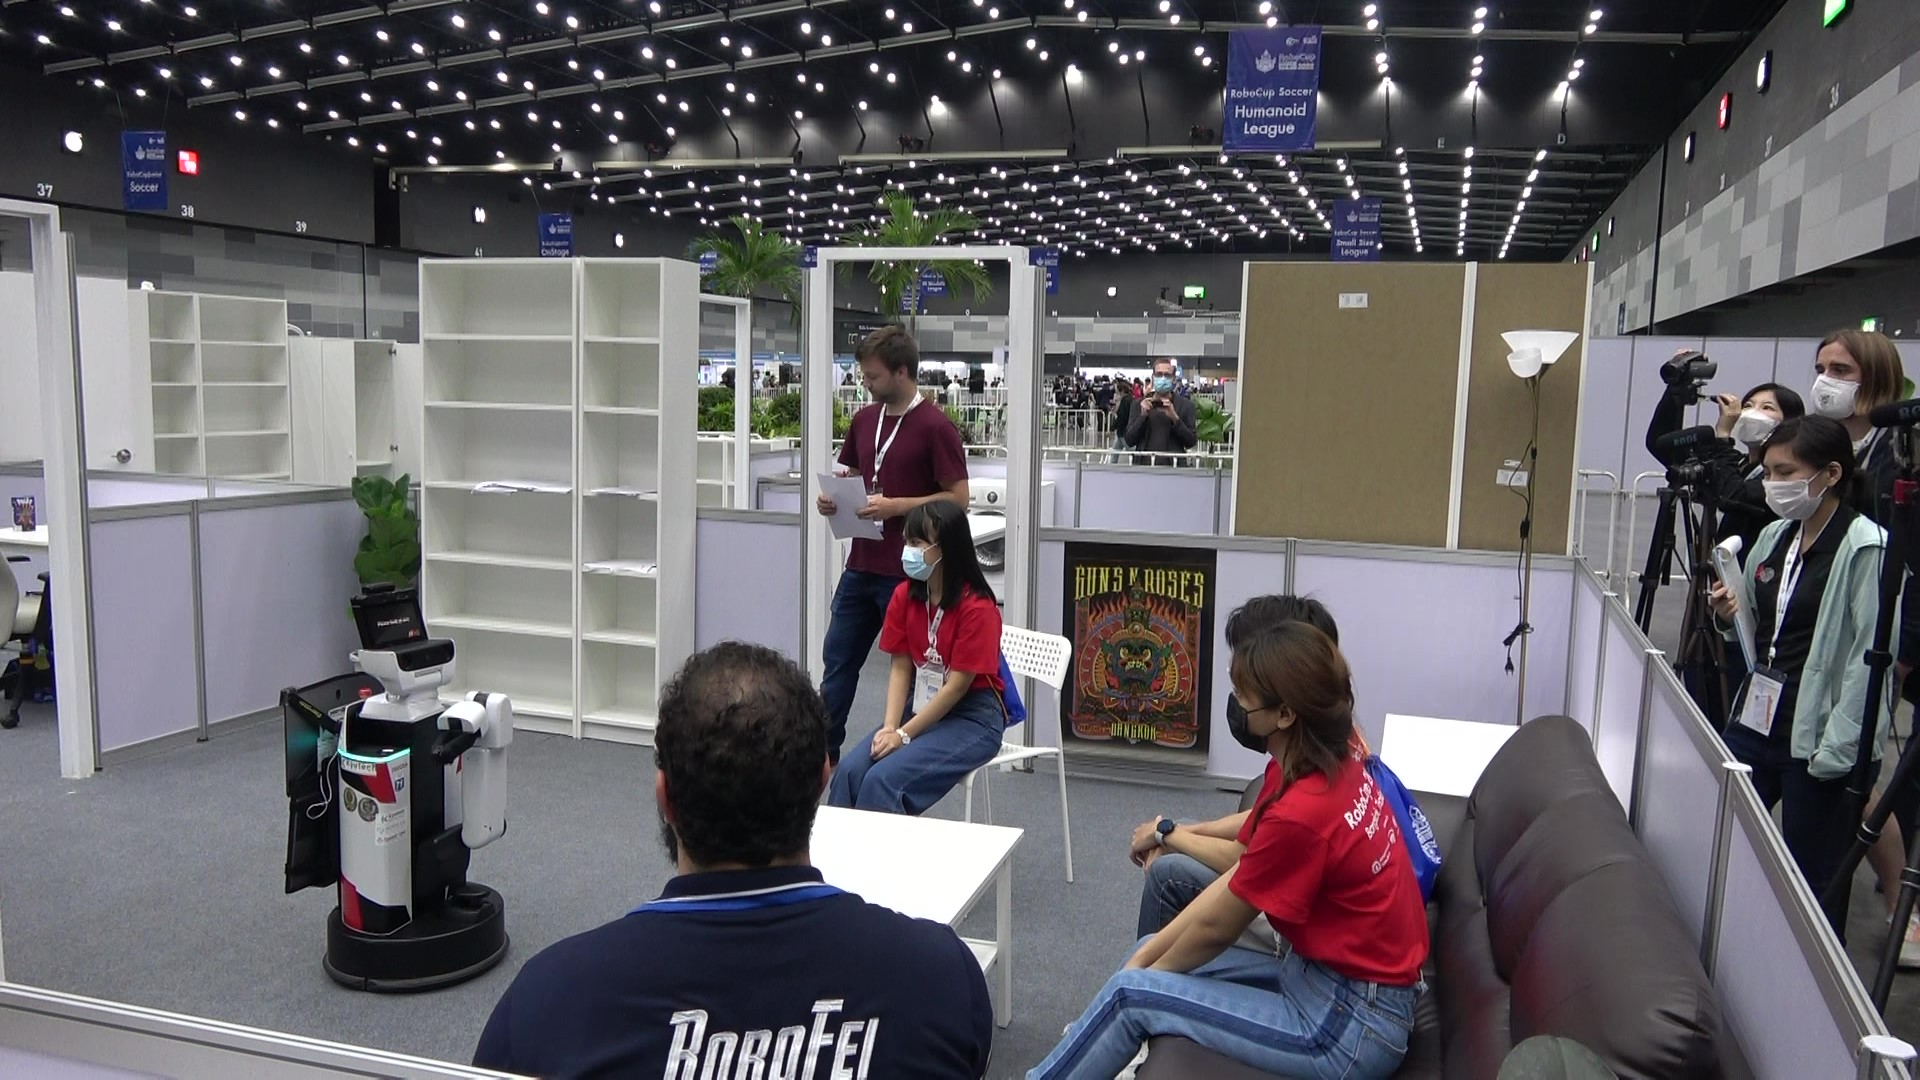
\includegraphics[height=2.2cm]{images/robocup/FMM_onsite_overview_3.jpg}
  \caption{FMMが行われた実際の会場}
  \label{onsite_overview_1}
\end{figure}
% 提案手法をHSRに実装し,2022年7月にバンコクで行われたRoboCup@Homeで性能評価を行った.
我々は2022年7月にバンコクで行われたRoboCup@Homeに参加し,提案手法の評価と現地環境における音声認識の精度検証を行った.
RoboCup@HomeではHSRの制御用にPCを1台使用することが認められているため,以下のようなPCを使用した.
CPU:Intel core i7-7820HK, GPU:Geforce RTX 1080,メモリ:32GB,OS:Ubuntu18.04.
また,PCとHSRの通信にはRobot Operating System \cite{ros_wiki}を用いている.
% 4つのルームがある中で,FMMはリビングルームにて実施された.

実際に使用されたリビングルームの概略図を図\ref{robocup_field}に,競技中の様子を図\ref{onsite_overview_1}に示す.
% また,現地環境における音声認識の精度検証も併せて行った.
% RoboCup@Homeで使用される名前は,アメリカで一般的に用いられる名前からランダムに決定される.
% そこで,アメリカで一般的に使用されている名前から男女それぞれ11個選出し,
% 本番に近い環境で話者やノイズの強弱を変化させながら各名前を4度ずつ読み上げ,計88個の検証データを作成し評価を行った.

% 本研究で使用したPCは,CPU:Intel core i7-7820HK, GPU:Geforce RTX 1080,メモリ:32GB,OS:Ubuntu18.04である.
% RoboCup@HomeではHSRの制御用にPCを1台使用することが認められているため,以下のPCを使用した.
% CPU:Intel core i7-7820HK, GPU:Geforce RTX 1080,メモリ:32GB,OS:Ubuntu18.04.
% また,PCとHSRの通信にはRobot Operating System \cite{ros_wiki}を用いている.

\section{競技結果}

\subsection{音声認識の性能評価}
始めに,提案手法における音声認識の性能評価を行った.
実験に際して,アメリカで一般的に使用されている名前から男女それぞれ11個を選出し,
本番に近い環境で話者やノイズの強弱を変化させながら4度ずつ読み上げ,計88個のデータを作成した.
% RoboCup@Homeで使用される名前は,アメリカで一般的に用いられる名前からランダムに決定される.
% そこで,
表\ref{voice_recognition_result}に,ノイズ除去と辞書指定の有無による認識結果を示す.
ノイズ除去と辞書指定を行っていないの場合の精度は13.6\%であったが,辞書指定を行うことで55.7ポイント向上し69.3\%となった.
% 辞書指定なしでの精度は約10\%であったが,辞書指定ありでは約70\%であった.
加えてノイズ除去を行うことによって,精度が2.3ポイント向上し71.6\%で最も高くなった.
しかし,辞書指定を行っていない場合では,ノイズ除去を行うことで精度が3.4ポイント低下した.
% また,辞書指定を行った場合でも,ノイズ除去を行ったことでかえって認識に失敗するデータが3個あることが確認できた.
% また,辞書指定を行った場合でも,ノイズ除去を行ったことでかえって認識に失敗するデータがあることも確認できた.
\begin{table}[b]
	\centering
	\caption{音声認識の精度}
	\begin{tabular}{|c|c|c|}
	\hline
	辞書指定                & ノイズ除去 & 認識精度(\%)          \\ \hline
	\multirow{2}{*}{なし} & なし    & 13.6          \\ \cline{2-3}
	                    & あり    & 10.2          \\ \hline
	\multirow{2}{*}{あり} & なし    & 69.3          \\ \cline{2-3}
	                    & あり    & \textbf{71.6} \\ \hline
	\end{tabular}
	\label{voice_recognition_result}
\end{table}

\subsection{FMMの結果}
我々はRoboCup@HomeでFMMを2度トライし,性能評価を行った.
1度目のトライでは部屋中央へのナビゲーションに失敗し,ゲストから遠い位置にHSRが停止してしまった.
% の目的地がゲストから遠い位置であったため,
% その結果,不鮮明・不明瞭な画像を取得することとなった.
それでも,人物検出と3次元の位置推定は正常に動作したが,各ゲストの顔画像が非常に低い解像度となってしまった.
そのため属性推定が正常に動作せず,ゲストの2人が男性で2人が女性であったが,全員を女性と判定した.
また,音声認識では認識結果を得ることが出来ず,QRコードによるバイパスを用いた.
結果としては,ヘッドディスプレイに表示した人物画像が不明瞭であったため,人物報告,位置報告の両方が認められず0点であった.

% 2度目のトライは,1度目にあったナビゲーションの目的地が遠いという問題点を修正してから行った.
2度目のトライは,1度目にあったナビゲーションの問題点を修正してからトライした.
% その結果,ゲストをより近い位置から認識することが出来たため,鮮明な画像を得ることができ,属性推定も間違いなく動作した.
その結果,ゲストをより近い位置から認識することが出来たため,取得画像が鮮明になり属性推定も間違いなく動作した.
しかし,音声認識部においてはゲストの前までナビゲーションを行うことは出来たが,名前を聞き取ることは出来ず,再度QRコードのバイパスを使用することとなった.
2度目のトライにおいて,フィールド内の状況を説明するために生成した画像を図\ref{result_FMM_2}に示す.
\begin{figure}[t]
  \centering
  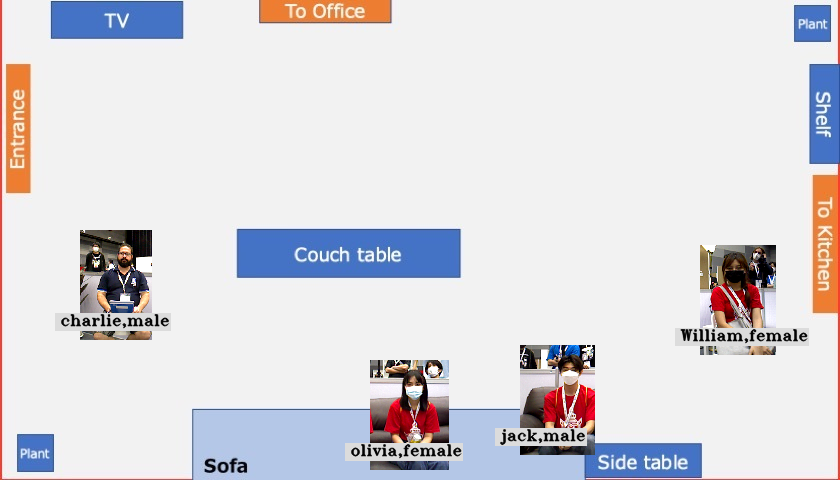
\includegraphics[width=7cm]{images/FMM/mapimage.png}
  \caption{2回目のトライで作成したマップイメージ}
  \label{result_FMM_2}
\end{figure}
今回のトライでは,ゲストは図\ref{onsite_overview_1}(b)の通りに座っており,生成画像では全員の座っている位置を間違いなく報告できている.
更に,性別と名前も正解しているため,結果として満点の1000点を獲得した.
% 参加チームごとのFMMで獲得した点数を表\ref{fmm_points_eachcheam}にまとめる.
% \begin{table}[h]
% \begin{tabular}{ll}
%                              & Find My Mates \\
% Hibikino-Musashi@Home (ours) & \textbf{1000} \\
% Tech United Eindhoven        & \textbf{1000} \\
% Team ORIon                   & 0
% \end{tabular}
% \label{fmm_points_eachcheam}
% \end{table}


\section{考察}

\subsection{ノイズ除去}
本研究では,音声認識の精度向上を目的としてノイズ除去を適用した.
その結果,検証データ全体では認識精度が向上していることが確認できた.
しかし,検証データ88個のうち3個のデータにおいては,ノイズ除去を行うことでかえって認識に失敗するという結果となった.
このことから,ノイズ除去が必ずしも認識精度の向上に繋がるわけではないということが分かった.
% しかし,全体の認識精度は向上しているため,ノイズ除去は音声認識に有効な手段であると言える.
今後は,音声認識にとってより有効なノイズ除去の手法について検討を進めていく必要がある.

\subsection{音声認識}
% 今回の現地実験では,FMMを2回実施したが,いずれも音声認識の結果を得ることは出来なかった.
我々はRoboCup@Home2022でFMMを2度実施したが,音声認識が未検出となり結果を得ることができなかった.
% 原因として,音声認識中のGraphical User Interface(GUI)が発話者に伝わっておらず,音声認識時間外に発話されたことと,発話者の声量が小さく認識が困難であったことが考えられる.
1つ目の原因として,音声認識時間外に発話されたことが挙げられる.
HSRはマイクとスピーカが別デバイスであるため,HSRが発話している間に音声認識を行うと,HSRの音声もマイクに入力されてしまう.
% また,本研究で実装した音声認識はゲストの発話状態にかかわらず一定時間のみ行うため,発話のタイミングが音声認識の結果に大きく影響してしまう.
また,本研究で実装した音声認識はゲストの発話状態にかかわらず一定時間のみ行うため,認識精度が発話タイミングによって大きく変動してしまう.
% そこで,HSRのヘッドディスプレイに認識中を示すようなGUIを作成していたが,このGUIが発話者に伝わっておらず認識時間外に発話されることがあった.
そこで,HSRのヘッドディスプレイに発話のタイミングを誘導するような表示をしていたが,この表示が発話者に伝わっておらず,認識時間外に発話されることがあった.

2つ目の原因として,発話者の近くまでナビゲーション出来なかったことが挙げられる.
バンコクで実際に使用された会場では,ゲストの座っているソファの手前にテーブルがあったため,ゲストの手前まで移動することが出来なかった.
そのため,遠い位置からの音声認識となり,マイクに入力される発話者の音声が非常に小さくなってしまった.
このことから,音声認識の結果を得ることが困難であったと考えられる.
今後は,発話のタイミングに応じて音声認識を開始,終了するような機能を作成する必要がある.
また,発話者の音声が小さいことも考慮して,音声強調\cite{voice_enhancement_1, voice_enhancement_2}の技術を活用する必要がある.

\subsection{位置推定}
提案手法では,HSRが事前に取得したマップのどこがフィールドで,どこに椅子やソファがあるのかという情報を事前に与える必要がある.
RoboCup@Homeのルールでは,事前に部屋の情報が公開されることになっているが,本大会では椅子の位置が何度も変更されたため,対応が困難であった.
% 今後はロバスト性の高い3次元的な物体認識手法\cite{sun2022onepose}を用いて,家具の位置変化に頑健なシステムを構築する必要があると考える.
今後は3次元的な物体認識手法\cite{sun2022onepose}を用いて,家具の位置変化に頑健なシステムを構築する必要があると考える.


\section{結論}
本研究では,国際的な競技会であるRoboCup@Homeで行われるFMMに向けての解法を提案し,実機実装を通してその性能評価を行った.
競技会では2回目のトライで満点を獲得し,提案手法の有効性を示した.
一方で,音声認識やナビゲーションに関しての課題点も見つかったため,今後はこれらの課題を解決するために研究を続けていく必要がある.

\begin{thebibliography}{99}
%\small

\bibitem{robocup_hp}
RoboCup@Home. \url{https://www.robocup.org/domains/3}, (Accessed 2022-09-01).

\bibitem{hsr_paper}
% T. Yamamoto, K. Terada, A. Ochiai, F. Saito, Y. Asahara, and K. Murase, Development of Human Support Robot as the research platform of a domestic mobile manipulator, ROBOMECH Journal, Vol. 6, Art. no. 4, 2019.
T. Yamamoto, K. Terada, A. Ochiai, F. Saito, Y. Asahara and K. Murase, “Development of Human Support Robot as the research platform of a domestic mobile manipulator,” ROBOMECH Journal, Vol. 6, Art. no. 4, (2019).

% \bibitem{vosk}
% Author, A., Author, B.:
% JSAI SIGs Conference Paper Format Sample,
% {\it International Journal of Examples}, Vol.~19, No.~4, pp.~1--2 (2007)


% \bibitem{yolo}
% 第一著者, 第二著者:
% 人工知能学会研究会原稿フォーマットサンプル,
% {\it International Journal of Examples}, Vol.~19, No.~4, pp.~1--2 (2007)

\bibitem{google_speech_api}
Google Speech-to-Text. \url{https://cloud.google.com/speech-to-text}, (Accessed 2022-09-03).

\bibitem{amazon_speech_api}
Amazon Transcribe \url{https://aws.amazon.com/jp/transcribe/}, (Accessed 2022-09-03).

\bibitem{CSRA}
K. Zhu and J. Wu, "Residual Attention: A Simple but Effective Method for Multi-Label Recognition," 2021 IEEE/CVF International Conference on Computer Vision (ICCV), pp. 184-193 (2021).

\bibitem{vosk_hp}
α cephei Vosk Offline speech recognition. \url{https://alphacephei.com/vosk/}, (Accessed 2022-09-04).

\bibitem{sainburg2020finding}
% Sainburg, T., Thielk, M., and Gentner, T. Q.,
T. Sainburg, M. Thielk and T. Q Gentner,
% Sainburg, Tim and Thielk, Marvin and Gentner, Timothy Q
“Finding, visualizing, and quantifying latent structure across diverse animal vocal repertoires,”
{\it Public Library of Science PLoS computational biology},
Vol.16,
No.10,
pp.e1008228,
(2020).

\bibitem{light-openpose}
D. Osokin, "Real-time 2d multi-person pose estimation on cpu: Lightweight openpose." arXiv preprint arXiv:1811.12004 (2018).
% Osokin, Daniil. "Real-time 2d multi-person pose estimation on cpu: Lightweight openpose." arXiv preprint arXiv:1811.12004 (2018).

% \bibitem{rtabmap}
% M. Labbé and F. Michaud, “RTAB-Map as an Open-Source Lidar and Visual SLAM Library for Large-Scale and Long-Term Online Operation,” in Journal of Field Robotics, vol. 36, no. 2, pp. 416–446, (2019).

\bibitem{ros_wiki}
Robot Operating System Wiki. \url{https://wiki.ros.org/}, (Accessed 2022-09-01).

\bibitem{voice_enhancement_1}
  % author = {Serrà, Joan and Pascual, Santiago and Pons, Jordi and Araz, R. Oguz and Scaini, Davide},
J. Serrà, S. Pascual, J. Pons, R. O. Araz and D. Scaini, “Universal Speech Enhancement with Score-based Diffusion,” arXiv (2022).

\bibitem{voice_enhancement_2}
% Simon Welker, Julius Richter and Timo Gerkmann. "Speech Enhancement with Score-Based Generative Models in the Complex STFT Domain", ISCA Interspeech, 2022.
% Welker, S., Richter, J., and Gerkmann, T. "Speech Enhancement with Score-Based Generative Models in the Complex STFT Domain", ISCA Interspeech, (2022).
S. Welker, J. Richter, and T. Gerkmann, "Speech Enhancement with Score-Based Generative Models in the Complex STFT Domain", ISCA Interspeech, (2022).

% \bibitem{omni3d}
% % Garrick Brazil and Julian Straub and Nikhila Ravi and Justin Johnson and Georgia Gkioxari, “Omni3D: A Large Benchmark and Model for {3D} Object Detection in the Wild,” arXiv:2207.10660, (2022).
% G. Brazil, J. Straub, N. Ravi, J. Johnson and G Gkioxari, “Omni3D: A Large Benchmark and Model for {3D} Object Detection in the Wild,” arXiv:2207.10660, (2022).

\bibitem{sun2022onepose}
% Sun, Jiaming and Wang, Zihao and Zhang, Siyu and He, Xingyi and Zhao, Hongcheng and Zhang, Guofeng and Zhou, Xiaowei, “OnePose: One-Shot Object Pose Estimation without CAD Models,” Conference on Computer Vision and Pattern Recognition(CVPR), (2022).
J. Sun, Z. Wang, S. Zhang, X. He, H. Zhao, G. Zhang and X. Zhou, “OnePose: One-Shot Object Pose Estimation without CAD Models,” Conference on Computer Vision and Pattern Recognition(CVPR), (2022).

\end{thebibliography}

\end{document}
